\section{Uvod}

\subsection{\textit{Commodore 1541}, \textit{5.25" flopi disketa} i \textit{D64 fajl}}
\textit{Commodore 1541} je čitač \textit{5.25" flopi disketa} korićenih u radu sa \textit{Commodore 64} računarima. Razvijen je u Kanadi od strane kompanije \textit{Commodore}, 1982. godine. Ovaj čitač imao je jednu glavu za čitanje i pisanje sa \textit{Commodore 64} računarom i bio je povezan sa njim preko \textit{serial bus-a}. Imao je dve lapmpice, zelenu koja je označavala da je uređaj uključen u struju i crvenu koja se palila kada uređaj radi \cite{Commodore1541Text}. Izgled čitača prikazan je na slici \ref{img:commodore1541}.
\begin{figure}[ht]
\begin{center}
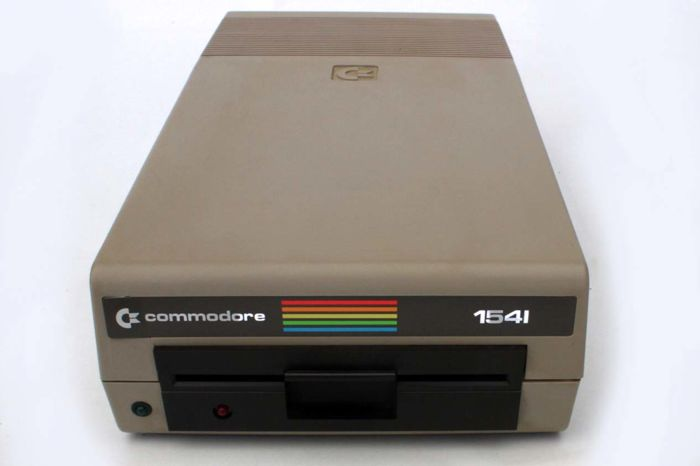
\includegraphics[width=\textwidth]{img/Commodore1541.jpg}
\caption[Commodore 1541 \textit{(preuzeto \cite{Commodore1541})}]{Commodore 1541}
\label{img:commodore1541}
\end{center}
\end{figure}

Originalna \textit{5.25" flopi disketa} ili \textit{miniflopi} bio je magnetni medijum format koga je 1976. godine predstavio \textit{Shugart Associates} kao zamenu za \textit{8-inčnu disketu} koja se smatrala prevelikom za novije računare \cite{5.25Flopi}. Izgled diskete prikazan je na slici \ref{img:flopi}.

Osnovni oblik ove diskete imao je 35 kružnih traka dok je postojala i verzija sa 40 traka na kojima su bili raspoređeni sektori od po 256 bajta. Trake su imale različit broj sektora i bile su raspoređene od spolja ka unutra, odnosno prva traka je bila bliža spoljašnjoj ivici i imala je najviše sektora, dok je poslednja traka bila bliža unutrašnjem prstenu diskete sa najmanje sektora. Broj sektora po trakama je prikazan u tabeli \ref{tab:sektor_traka}.

\begin{figure}[ht]
\begin{center}
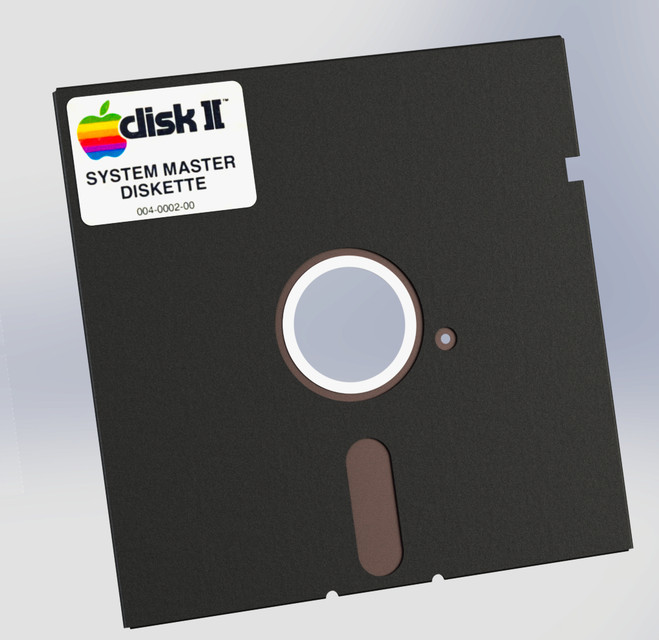
\includegraphics[width=\textwidth]{img/Flopi.jpg}
\caption[5.25" flopi disketa \textit{(preuzeto \cite{Flopi})}]{5.25" flopi disketa}
\label{img:flopi}
\end{center}
\end{figure}

\begin{table}[h!]
\begin{center}
\begin{tabular}{ | c | c| c | c | } 
\hline
Traka & Sektori/traka & Ukupno Sektora & Skladište u bajtima \\
\hline
\hline
1-17 & 21 & 357 & 7820 \\
\hline
18-24 & 19 & 133 & 7170 \\
\hline
25-30 & 18 & 108 & 6300 \\
\hline
31-35 & 17 & 85 & 6020 \\
\hline
\end{tabular}
\end{center}
\caption{Broj sektora po traci originalne \textit{5.25" flopi diskete}}
\label{tab:sektor_traka}
\end{table}

Traka 18 predstavlja glavnu traku sa svojih 19 sektora. Nulti sektor ove trake čuva \textbf{BAM}(eng. Block Availability Map), ime i id flopi diskete dok ostali sektori sadrže podatke. \textbf{BAM} je struktura podataka koja prati koji sektori traka su slobodni a koji zauzeti. Sektor u kome je smešten \textbf{BAM} je formiran po posebnom šablonu. \textbf{BAM} za prvu traku smešten je od 4-7 bajta nultog sektora. Prvi bajt \textbf{BAM-a} govori ukupan broj slobodnih sektora, dok preostala tri govore koji sektori su slobodni a koji popunjeni. Svaka naredna 4 bajta predstavljaju \textbf{BAM} za narednu traku flopi diskete. 128 bajt čuva ime flopi diskete dok 146 bajt čuva id diskete.

Podaci su uvek smešteni počevši od prvog sektora, ukoliko je reč o direktorijumima pomeranje se vrši za tri sektora pa je nastavak na četvrtom sektoru dok se za smeštanje fajlova pomeranje vrši za deset sektora i tada je nastavak na desetom sektoru. Sektori su popunjeni po šablonu, prva dva bajta sektora govore o lokaciji sledeće trake/sektora. Kada dođemo do kraja direktorijuma vrednost prvog bajta je 00.

\textit{D64 fajl} je najšire podržani i dobro definisan format koji predstavlja elektronsku bajt predstavu \textit{5.25"flopi diskete} za \textit{Commodore 64} računare. Standardni \textit{D64 file} ima 174848 bajtova, 683 sektora sa po 256 bajta i on oslikava originalnu \textit{5.25" flopi disketu} sa 35 traka.  Postoji i verzija ovog fajla sa 196608 bajtova,768 sektora sa po 256 bajta koja oslikava verziju \textit{5.25" flopi diskete} sa 40 traka.

Na kraju \textit{D64 fajla} mogu se naći dodatni bajtovi, koji govore koji sektori imaju grešku. Ukoliko se na kraju fajla ne pojave bajtovi to znači da su svi sektori ispravni. Svaki bajt je vezan za po jedan sektor odnosno koliko sektora flopi disketa ima toliko će imati i bajtova na kraju fajla ukoliko taj fajl ima grešku u nekom od sektora. U zavisnosti od broja traka i broj dodatnih bajtova se menja i to za 35 traka 689 bajtova dok je za 40 traka 768 bajtova. Ukoliko je vrednost bajta postavljena na 1 to znači da korespodentni sektor nema grešku \cite{D64}. Veličina fajlova u zavisnosti od dodatnih bajtova je prikazana u tabeli \ref{tab:error_velicina}.
\begin{table}[h!]
\begin{center}
\begin{tabular}{ | c | c |} 
\hline
Tip diskete & Veličina(bajt) \\
\hline
\hline
35 traka, bez grešaka & 174848 \\
\hline
35 traka, 689 bajtova greški & 175531 \\
\hline
40 traka, bez grešaka & 196608 \\
\hline
40 traka, 768 bajtova greški & 197376 \\
\hline
\end{tabular}
\end{center}
\caption{Veličina fajla u zavisnosti od dodatnih bajtova}
\label{tab:error_velicina}
\end{table}
